\documentclass[letterpaper,12pt]{article} 
\usepackage[utf8]{inputenc}
%\usepackage[mathletters]{ucs}
\usepackage[backend=biber,style=apa]{biblatex}
\addbibresource{references.bib} %Imports bibliography file
% Language setting
% Replace `english' with e.g. `spanish' to change the document language
\usepackage[spanish]{babel}
% Set page size and margins
\usepackage[a4paper,top=2cm,bottom=2cm,left=3cm,right=3cm,marginparwidth=1.75cm, headheight=64pt]{geometry}
\usepackage{mathptmx}
\usepackage{amsmath}
\usepackage{amsfonts}
\usepackage{amssymb}
\usepackage[T1]{fontenc}
\usepackage{gentium}
\usepackage{float}
\usepackage{termcal}
\usepackage[table]{xcolor}
\usepackage{needspace}
\usepackage{titlesec}
\usepackage{enumitem}
\usepackage{graphicx} % Required for inserting images
\usepackage{wrapfig}
\usepackage{enumitem}
\usepackage{fancyhdr}
\usepackage{float}
\usepackage{eurosym}
\usepackage{color}
\usepackage{titling}
\usepackage{lipsum}
\usepackage{tocbibind}
\usepackage{datetime2}
\usepackage[colorlinks=true,linkcolor=black,anchorcolor=black,citecolor=black,filecolor=black,menucolor=black,runcolor=black,urlcolor=black]{hyperref}
%tikz image
\usepackage{amsmath}
\usepackage{color,pxfonts,fix-cm}
\usepackage{latexsym}
\usepackage{pict2e}
\usepackage{wasysym}
\usepackage{tikz}
\usetikzlibrary{mindmap, trees}
\usepackage{adjustbox}
\usepackage{tabularx}
\usepackage{ragged2e}
\usepackage{csquotes}
\usepackage{pdfpages}

% Set section and subsection titles to font size 12
\titleformat*{\section}{\normalfont\fontsize{12}{14}\bfseries}
\titleformat*{\subsection}{\normalfont\fontsize{12}{14}\bfseries}

%%% Para las cabeceras
\newcommand{\hsp}{\hspace{20pt}}
\newcommand{\HRule}{\rule{\linewidth}{0.5mm}}
\headheight=50pt

\newcommand{\vacio}{\textcolor{white}{UCB-SC}}

%\DTMlangsetup[es-ES]

\title{Smoke Detector Cam}
\author{
    Leonardo Achá Boiano \\
    Bruno Ramiro Rejas Montero}


\title{Propuesta de Proyecto:\\Smoke Detector Cam}

\begin{document}

\maketitle

\needspace{3cm}
\section{Introducción}

El presente informe tiene como objetivo presentar la propuesta del proyecto "Smoke Detector Cam". Este proyecto tiene como finalidad desarrollar un sistema inteligente basado en una cámara con capacidad de detección de humo y fuego para contribuir a la prevención y mitigación de incendios, así como para promover ambientes libres de humo de tabaco, en cumplimiento con la recientemente promulgada ley de control del tabaco en Bolivia.

\needspace{3cm}
\section{Antecedentes del problema}
El tabaquismo es una epidemia mundial con graves consecuencias para la salud, la sociedad y la economía. En Bolivia, aproximadamente el 21,9\% de los hombres y alrededor del 9\% de las mujeres consumen tabaco diariamente(\cite{BoliviaTobaccoControlLaw}). Además, un preocupante 46,6\% de los jóvenes están expuestos al humo de tabaco ajeno, y cada año más de 4.600 bolivianos y bolivianas pierden la vida debido a enfermedades relacionadas con el consumo de tabaco.

Para abordar esta preocupante situación, se promulgó una importante ley de control del tabaco en Bolivia. Misma que estableció que todos los espacios cerrados de acceso público y lugares de trabajo deben ser 100\% libres de humo de tabaco, protegiendo así a toda la población de los riesgos asociados a la exposición al humo de segunda mano. Según lo reportado por la Organización Mundial de la Salud (OMS) se estima que alrededor de 8 millones de personas mueren cada año debido al tabaquismo, de las cuales 7 millones de muertes son atribuidas al consumo directo de tabaco y 1 millón de muertes son causadas por el humo de tabaco ajeno.

Además de los impactos en la salud, el tabaquismo también genera una significativa carga económica, con la OMS estimando que la economía mundial tiene que soportar más de USD 500 mil millones cada año debido a problemas relacionados con el tabaquismo.

La vigilancia basada en inteligencia artificial de las áreas de no fumar para detectar fumadores como posibles infractores es esencial(\cite{Khan2022b}). Al tener una solución automatizada y precisa, las autoridades pueden aplicar medidas correctivas oportunas y fomentar el cumplimiento de las regulaciones, mejorando así la calidad de vida y el bienestar general en el contexto de ciudades inteligentes.
Esta solución puede contribuir significativamente al monitoreo y prevención del consumo de tabaco en espacios donde está prohibido fumar.

\needspace{3cm}
\section{Identificación del problema}

El tabaquismo representa un grave problema de salud pública en Bolivia, con un alto número de fumadores y personas expuestas al humo de segunda mano. Es esencial implementar medidas efectivas para asegurar ambientes libres de humo y promover el cumplimiento de la ley de control del tabaco.

\needspace{4cm}
\section{Justificación} 
\subsubsection{Justificación Social} 
La adopción de "Smoke Detector Cam" se basa en un compromiso con la responsabilidad social y la creación de ambientes más seguros y saludables en la sociedad. Este sistema, diseñado para detectar personas fumando en lugares públicos y privados, cumple un papel crucial al promover el respeto de las convenciones sociales que prohíben fumar en espacios cerrados. Al hacerlo, contribuye a la creación de entornos libres de humo, mejorando la calidad del aire y protegiendo la salud de quienes comparten estos lugares. 
\subsubsection{Justificación Legal} 
La implementación del sistema de detección de humo y fuego denominado "Smoke Detector Cam" se basa en la necesidad de cumplir con las regulaciones legales que prohíben el acto de fumar en recintos cerrados. Estas leyes y normativas tienen como objetivo principal resguardar la salud pública y reducir los riesgos de incendios originados por el consumo de tabaco en espacios confinados. La introducción de este sistema garantizará el estricto cumplimiento de dichas disposiciones legales al identificar y disuadir cualquier actividad de fumar en lugares donde la ley prohíbe expresamente esta conducta.
\subsubsection{Justificación Ambiental} 
Desde una perspectiva ambiental, la implementación de "Smoke Detector Cam" 
 encuentra su justificación en su capacidad para contribuir a la preservación del entorno natural. Este sistema de detección temprana no solo preserva vidas humanas, sino que también juega un papel fundamental en la prevención de incendios, especialmente en áreas con vegetación. Los incendios, tanto forestales como urbanos, pueden tener un impacto devastador en los ecosistemas locales, aumentar la emisión de contaminantes atmosféricos y reducir la biodiversidad. Al detectar a las personas fumando en áreas con vegetación, "Smoke Detector Cam" minimiza el riesgo de incendios, lo que a su vez contribuye de manera significativa a la conservación del entorno natural y a la mitigación de los efectos del cambio climático.
\subsubsection{Justificación Academica} 
La justificación académica para la implementación de "Smoke Detector Cam" se basa en su capacidad para respaldar la investigación y el proceso de aprendizaje en diversas áreas. Este sistema generará valiosos datos sobre la identificación de personas fumando en diferentes entornos, lo que puede servir como una fuente rica de información para instituciones académicas y centros de investigación. Además, la tecnología empleada en este sistema no solo abrirá oportunidades para la colaboración entre instituciones educativas y la industria en seguridad y detección de comportamientos relacionados con el tabaco, sino que también podría llevar a avances en sistemas de refrigeración más eficientes. Esto enriquecería el entorno académico y permitiría la formación de profesionales con conocimientos especializados en seguridad, detección de comportamientos y sistemas de refrigeración de vanguardia.

\needspace{3cm}
\section{Objetivos}
El proyecto "Smoke Detector Cam" tiene los siguientes objetivos:

\subsection{Objetivo General}
Desarrollar el mecanismo de movimiento del sistema embebido "Smoke Detector Cam" para la detección temprana de humo y fuego en ambientes cerrados, con el propósito de contribuir a la prevención y mitigación de incendios y promover ambientes libres de humo de tabaco en cumplimiento de la ley de control del tabaco en Bolivia.

\needspace{3cm}
\subsection{Objetivos Específicos}
\begin{itemize}
\item Desarrollar "Smoke Detector Cam" con sensores de humo, cámara, refrigeración y batería, teniendo en cuenta limitaciones de espacio y fabricación.
\item Crear el cuerpo de la cámara con software CAD para impresión 3D a gran escala, enfocándose en resistencia, durabilidad y adaptabilidad a diferentes entornos cerrados.
\item Simular el sistema de refrigeración planificado para garantizar el correcto funcionamiento de los componentes electrónicos sin afectar la apariencia visual, utilizando herramientas de análisis de ingeniería asistida por computadora (CAE).
\needspace{4cm}
\item Aplicar el método de gestión de proyectos de cinco pasos de la literatura académica (\cite{Ulrich2012}), que incluye identificar oportunidades, evaluar proyectos, asignar recursos y tiempo, finalizar la planificación del anteproyecto y reflexionar sobre los resultados y el proceso.
\end{itemize}

\needspace{3cm}
\section{Detalle mínimo de la propuesta}
El sistema "Smoke Detector Cam" será una cámara inteligente equipada con un algoritmo de inteligencia artificial que permitirá la detección temprana de humo y fuego en ambientes cerrados. Los detalles mínimos de la propuesta serán los siguientes:

El peso del producto será inferior a 250 g, lo que garantizará su portabilidad y facilidad de instalación en diversos entornos. Se prevé que la mayor parte del dispositivo sea desarrollado utilizando materiales de alta calidad como PLA o ABS, permitiendo su producción en masa a través de impresión 3D, lo que a su vez favorecerá la eficiencia y reducción de costos.

Las dimensiones del "Smoke Detector Cam" estarán por debajo de 200x110x100 mm, con el objetivo de optimizar su tamaño y permitir su instalación en espacios reducidos. Se planea reducir las dimensiones del primer prototipo en al menos un 30%, lo que mejorará su versatilidad y discreción.

En cuanto a las funcionalidades, el producto contará con 2DOF (Dos Grados de Libertad) para una cobertura amplia, además de conectividad WiFi y Bluetooth para facilitar su integración con otros sistemas de seguridad. La autonomía de la cámara será de al menos 1 hora, brindando un tiempo suficiente para una detección efectiva.

El algoritmo de detección de humo y fuego utilizará técnicas avanzadas de visión por computadora y aprendizaje profundo (deep learning), lo que permitirá analizar en tiempo real las imágenes captadas por la cámara. Cuando se detecte la presencia de humo o fuego, el sistema activará una alarma y enviará notificaciones a un centro de control y a las autoridades correspondientes, garantizando una respuesta rápida y eficiente ante situaciones de riesgo.

Se incluirán sensores para detectar el humo de tabaco en espacios cerrados, asegurando el cumplimiento de las regulaciones relacionadas con el control del tabaco. Cuando se identifique la presencia de humo de tabaco, el sistema enviará alertas a los responsables del lugar para que tomen las medidas adecuadas y mantengan un ambiente libre de humo.

\begin{table}[H]
\centering
\begin{tabular}{|l|l|}
\hline
\textbf{Característica} & \textbf{Especificacion}            \\ \hline
Peso                    & Inferior a 250 g                  \\ \hline
Materiales              & PLA o ABS                         \\ \hline
Dimensiones             & Inferior a 200x110x100 mm         \\ \hline
Grados de Movimiento    & 2DOF(X140° Y100°)                 \\ \hline
Conectividad            & Conexión WiFi, Bluetooth          \\ \hline
Autonomía               & Mínimo 1 hora                     \\ \hline
Algoritmo               & Visión por computadora, aprendizaje profundo  \\ \hline
Detección               & Humo y fuego en ambientes cerrados \\ \hline
Detección adicional     & Humo de tabaco en lugares cerrados, movimiento \\
\hline
\end{tabular}
\caption{Especificaciones de la cámara detectora de humo.}
\label{tab:fire_detection_specs}
\end{table}

Estas especificaciones garantizan un producto compacto, eficiente y con capacidades avanzadas de detección para mantener la seguridad en espacios públicos y garantizar el cumplimiento de las regulaciones sobre el consumo de tabaco.

\needspace{3cm}
\section{Boceto inicial de la propuesta}
\begin{figure}[H]
\centering
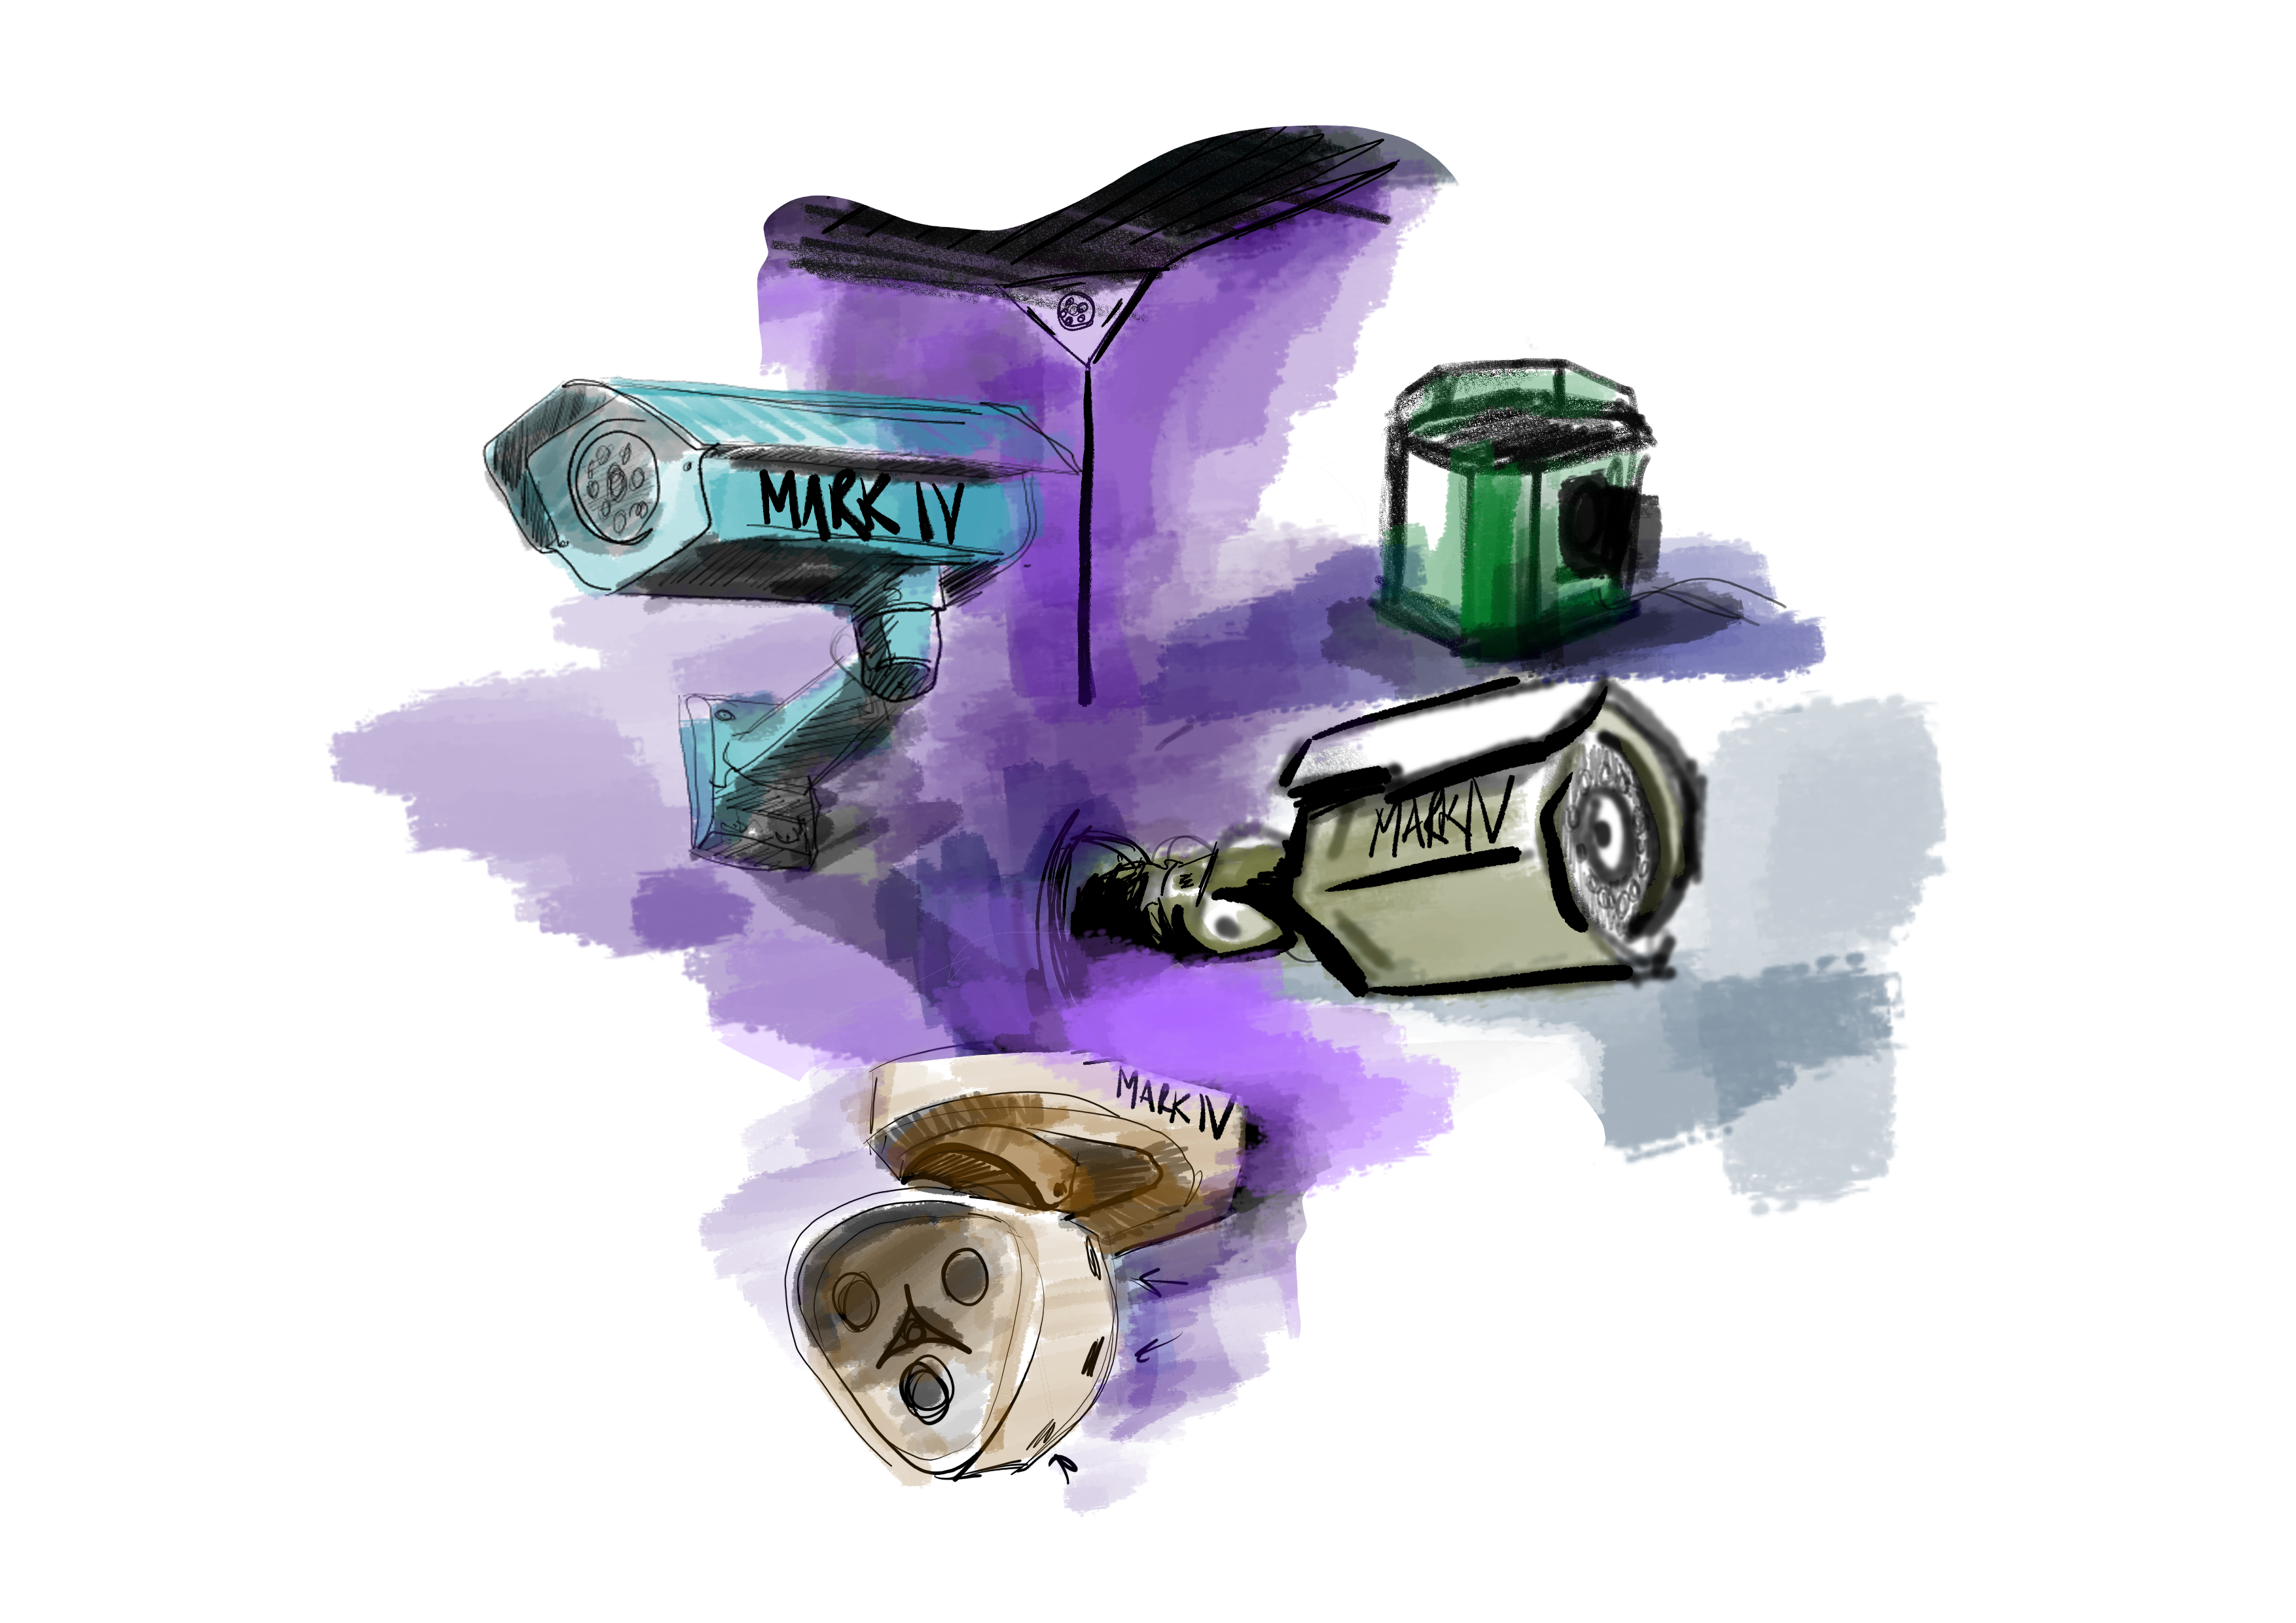
\includegraphics[width=0.70\linewidth]{media/concept_art.png}
\caption{\label{fig:concept_art}Arte conceptual del producto.}
\end{figure}

\needspace{3cm}
\section{Calendario}
\calwidth=15.5cm

% Few useful commands (our classes always meet either on Monday and Wednesday 
% or on Tuesday and Thursday)

\newcommand{\MWClass}{%
\calday[Monday]{\classday}
\calday[Tuesday]{\classday}
\calday[Wednesday]{\classday} 
\calday[Thursday]{\classday}  
\calday[Friday]{\classday}
\skipday\skipday % weekend (no class)
}

\newcommand{\TRClass}{%
\calday[Monday]{\classday}
\calday[Tuesday]{\classday} 
\calday[Wednesday]{\classday}
\calday[Thursday]{\classday} 
\calday[Friday]{\classday} % 
\skipday\skipday % weekend (no class)
}

\newcommand{\Holiday}[2]{%
\options{#1}{\noclassday}
\caltext{#1}{#2}
}

%\paragraph*{Calendario del Proyecto Smoke Detector Cam:}
\begin{center}
\begin{calendar}{08/28/2023}{15} % Semester starts on 1/11/2010 and last for 18

% weeks, including finals week
\setlength{\calboxdepth}{.25in}
\TRClass
% schedule

% Semana 5
\caltexton{0}{}

% Semana 6
\caltexton{6}{}

% Semana 7
\caltexton{5}{Presentación de propuestas de proyecto\cellcolor{green}}
\caltexton{7}{Objetivo 1.1}
\caltexton{10}{Objetivo 1.2}

% Semana 8
\caltexton{12}{}
\caltexton{15}{Metodo de los 5 pasos\cellcolor{green}}


% Semana 9 Examenes
\caltexton{16}{\cellcolor{red}}
\caltextnext{Objetivo 2.1\cellcolor{red}}
\caltextnext{\cellcolor{red}}
\caltextnext{\cellcolor{red}}
\caltextnext{\cellcolor{red}}
\caltexton{20}{Objetivo 1.4\cellcolor{red}}

% Semana 10 Examenes
\caltexton{21}{\cellcolor{red}}
\caltextnext{Objetivo 1.5\cellcolor{red}}
\caltextnext{\cellcolor{red}}
\caltextnext{\cellcolor{red}}
\caltextnext{\cellcolor{red}}

% Semana 11 Examenes
\caltexton{26}{\cellcolor{red}}
\caltextnext{\cellcolor{red}}
\caltextnext{\cellcolor{red}}
\caltextnext{\cellcolor{red}}
\caltextnext{\cellcolor{red}}

% Semana 12 Examenes
\caltexton{31}{\cellcolor{red}}
\caltextnext{\cellcolor{red}}
\caltextnext{\cellcolor{red}}
\caltextnext{\cellcolor{red}}
\caltextnext{\cellcolor{red}}

% Semana 13
\caltexton{36}{Objetivo 2.1\\Objetivo 2.2}

% Semana 14
\caltexton{41}{Objetivo 2.3}
\caltexton{44}{}

% Semana 15
\caltexton{47}{Objetivo 2.4}
\caltexton{49}{Proyecto Finalizado\cellcolor{green}}

% Semana 16 Examenes
\caltexton{50}{\cellcolor{red}}
\caltextnext{Objetivo 3.1\cellcolor{red}}
\caltextnext{\cellcolor{red}}
\caltextnext{\cellcolor{red}}
\caltextnext{\cellcolor{red}}

% Semana 17 Examenes
\caltexton{55}{\cellcolor{red}}
\caltextnext{Objetivo 3.2\cellcolor{red}}
\caltextnext{\cellcolor{red}}
\caltextnext{\cellcolor{red}}
\caltextnext{\cellcolor{red}}

% Semana 18
\caltexton{60}{}
\caltexton{61}{Objetivo 3.3}

% Semana 19 Finales
\caltexton{65}{\cellcolor{red}}
\caltextnext{\cellcolor{red}}
\caltextnext{\cellcolor{red}}
\caltextnext{\cellcolor{red}}
\caltextnext{\cellcolor{red}}

% Semana 20 Finales
\caltexton{70}{\cellcolor{red}}
\caltextnext{\cellcolor{red}}
\caltextnext{\cellcolor{red}}
\caltextnext{\cellcolor{red}}
\caltextnext{\cellcolor{red}}
\caltext{12/8/2023}{Ultimo día del semestre}

% Feriados
\Holiday{1/1/2023}{Año Nuevo (domingo) \cellcolor{orange}}
\Holiday{1/22/2023}{Estado plurinacional (domingo, festivo especial) \cellcolor{orange}}
\Holiday{2/20/2023}{Carnaval (lunes) \cellcolor{orange}}
\Holiday{2/21/2023}{Carnaval (martes) \cellcolor{orange}}
\Holiday{4/6/2023}{Semana Santa (jueves) \cellcolor{orange}}
\Holiday{4/7/2023}{Semana Santa (viernes) \cellcolor{orange}}
\Holiday{5/1/2023}{Día del Trabajador \cellcolor{orange}}
\Holiday{6/8/2023}{Corpus Christi (jueves) \cellcolor{orange}}
\Holiday{6/21/2023}{Año Nuevo aymara o andino \cellcolor{orange}}
\Holiday{8/7/2023}{Día de la Independencia \cellcolor{orange}}
\Holiday{11/2/2023}{Día de los Difuntos \cellcolor{orange}}
\Holiday{12/25/2023}{Navidad (lunes) \cellcolor{orange}}

\options{4/26/2023}{\noclassday} % finals week
\options{4/27/2023}{\noclassday} % finals week
\options{4/28/2023}{\noclassday} % finals week
\options{4/29/2023}{\noclassday} % finals week
\options{4/30/2023}{\noclassday} % finals week
\caltext{4/27/2023}{\textbf{Final Exam}}
\end{calendar}
\end{center}

\begin{minipage}{\linewidth}
    \subsection*{Objetivo 1: Diseñar el sistema electrónico de la cámara inteligente "Smoke Detector Cam"}

\begin{enumerate}[label=1.\arabic*]
    \item Identificar los componentes esenciales necesarios para el funcionamiento de la cámara inteligente, como sensores de humo, una cámara, sistemas de refrigeración y una batería.
    \item Investigar y seleccionar los componentes electrónicos y mecánicos adecuados que se adapten a las restricciones de espacio y las consideraciones de fabricación.
    \item Diseñar el esquema electrónico que incluya la interconexión de los componentes, considerando las necesidades de alimentación, control y comunicación.
    \item Utilizar software de diseño electrónico, como Eagle, KiCad o Altium, para crear un diseño de circuito impreso (PCB) que acomode los componentes de manera eficiente y cumpla con las restricciones de espacio.
    \item Realizar pruebas de prototipo para asegurarse de que los componentes funcionen correctamente y se comuniquen de manera efectiva.
\end{enumerate}

\subsection*{Objetivo 2: Desarrollar el cuerpo de la cámara utilizando software CAD}

\begin{enumerate}[label=2.\arabic*]
    \item Seleccionar un software CAD adecuado, como SolidWorks, AutoCAD o Fusion 360, para el diseño de la carcasa de la cámara.
    \item Diseñar la carcasa de manera que permita la integración de los componentes electrónicos, como la cámara y los sensores de humo, de manera eficiente tomando en cuenta las limitaciones y predisposiciones del método de manufactura seleccionado.
    \item Modelar el sistema de refrigeración seleccionado utilizando las técnicas de diseño pertinentes para maximizar la comparación y posterior análisis con mínimos recursos.
    \item Ajustar el diseño de la carcasa según sea necesario y realizar revisiones hasta obtener un diseño final satisfactorio.
\end{enumerate}

\subsection*{Objetivo 3: Realizar simulaciones del sistema de refrigeración}
\begin{enumerate}[label=3.\arabic*]
    \item Utilizar herramientas de análisis de ingeniería asistida por computadora (CAE), como ANSYS o COMSOL, para simular el rendimiento del sistema de refrigeración.
    \item Evaluar las temperaturas de funcionamiento de los componentes electrónicos y asegurarse de que estén dentro de los límites seguros.
    \item Optimizar el diseño del sistema de refrigeración según los resultados de las simulaciones.
\end{enumerate}
\end{minipage}

%\newpage
\printbibliography

\end{document}
